%!TEX root = ./main.tex
%!TEX encoding = UTF-8 Unicode
\chapter{description du format des instructions}
\label{chap:format}
La description du format des instructions se fait selon une structure arborescente, permettant de mutualiser au maximum le format commun entre chaque instruction. L'objectif ici est d'extraire à partir du format binaire d'une instruction, à la fois le type de l'instruction, ainsi que les différents opérandes. Au niveau du simulateur, cette étape constitue le \emph{décodage} de l'instruction.

Nous nous plaçons dans une première approche au cas des jeux d'instructions de taille fixe. La description sera ensuite étendue au cas des jeux d'instructions de taille variable dans la section \ref{sec:formatTailleVariable}.

\section{Architecture générale}
La description du format binaire va permettre de décoder une instruction à partir de son format binaire, tel qu'il est représenté dans le code objet du code applicatif à simuler. Dans un premier temps, il est nécessaire de fournir dans la section \texttt{default} au début de la modélisation l'information sur la taille des instructions:
\begin{lstlisting}
default {
    instruction := 16  -- default instruction size in bits
}
\end{lstlisting}
Dans cet exemple par exemple, la taille des instruction est sur 2 octets, ou un multiple de 2 octets pour les jeux d'instruction de taille variable. Par exemple, pour le \emph{HCS12}, les instruction ont une taille de 1 à 8 octets. Dans ce cas, il faut préciser \texttt{instruction := 8}.
La description du format décrit alors la manière de décoder le mot binaire dont la taille est fourni.

La structure générale des nœuds de description des format est de la forme:
\begin{lstlisting}
format <name> [etiquette]
  <formatBody>
end format
\end{lstlisting}

La partie \texttt{<formatBody>} est une succession d'éléments de type:
\begin{itemize}
\item \emph{étiquette};
\item appel à un autre nœud de type format;
\item structure de sélection, en utilisant le mot clé \texttt{select}. Voir section \ref{sec:formatSelect};
\item définition des opérandes. Voir section \ref{sec:operandeFormat}.
\end{itemize}

\subsection{Structure de sélection}
\label{sec:formatSelect}
L'utilisation de la sélection (différentes branches de l'arbre) se fait à travers l'instruction \texttt{select}, comme pour chaque vues de la description. 

Une sélection se fait sur un champ de bits extrait du format binaire d'une instruction:
\begin{lstlisting}
  select slice <field>
    case <masque> is <formatBody>
    case .. 
  end select
\end{lstlisting}

\subsubsection{partie \texttt{field}}
La partie \texttt{<field>} est utilisée pour désigner la partie du code de l'instruction qui permettra de distinguer différentes instructions. Soit par exemple les instructions \texttt{ADC} et \texttt{ADD} de l'AVR dont la représentation binaire est donnée sur la figure \ref{fig:selectFormat1}.

\begin{figure}[h]		%% select sur ADD et ADC
  \begin{center}
    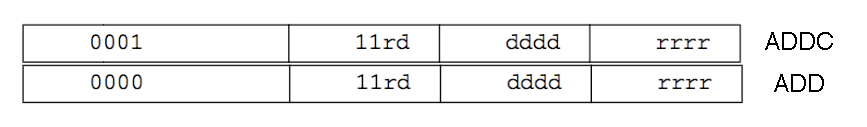
\includegraphics[width=0.8 \linewidth]{../common/images/selectFormat1.pdf}
    \caption{Codage binaire des instructions ADC et ADD de l'AVR (codage sur 16 bits).}
    \label{fig:selectFormat1}
  \end{center}
\end{figure}

dans ce cas, on pourrait par exemple utiliser une construction de la forme:
\begin{lstlisting}
  select slice {12}
    case 0 is ...
    case 1 is ...
  end select
\end{lstlisting}
En effet, uniquement le bit 12 permet de distinguer les 2 instructions. La partie \texttt{<field>} s'exprime de la même manière que l'accès à un champs de bit d'une variable (section \ref{sec:field}), en ajoutant la restriction d'utilisation à des valeurs numériques uniquement (pas d'expression):
\begin{lstlisting}
  select slice {12..10, 3..2} -- selection sur les bits 12 a 10 et 3 a 2, soit 5 bits au total
\end{lstlisting}
La taille du champ \texttt{<field>} doit être déterminée statiquement.

\subsubsection{partie \texttt{masque}}
La partie \texttt{masque} opère sur la valeur qui est transmise par la partie \texttt{<field>}, elle ne peut par conséquent pas avoir une taille supérieure au champ \texttt{<field>} (ceci engendre une erreur lors de la génération du simulateur).

La partie \texttt{masque} peut être soit une valeur numérique (comme dans l'exemple de la sous section précédente), soit un masque (voir section \ref{masque}). Lors de l'utilisation d'un masque, le caractère \texttt{-} peut être remplacé par un 0 ou un 1. Soit par exemple la description associées aux instructions de la figure \ref{fig:selectFormat1}, mais avec l'objectif de mutualiser ces 2 instructions:
\begin{lstlisting}
  select slice {15..10}
    case \m000-11 is .. -- cas pour ADD et ADC
    case ...
  end select
\end{lstlisting}
Dans ce cas, on va faire une sélection sur l'ensemble du code binaire de l'instruction à l'exception des opérande (\emph{opcode}). Le premier cas (\texttt{case}) sera pris pour les instructions dont les bits \texttt{15..10} sont \texttt{000011} (\texttt{ADD}) ou \texttt{000111} (\texttt{ADC}).

Il est aussi possible d'enrichir la partie \texttt{<masque>} en utilisant le mot clé \texttt{or}:
\begin{lstlisting}
select slice {7..0}
    case \x1B or \x1A or \x19 is ...
    ..
\end{lstlisting}
Cet exemple est extrait de la description du \emph{HCS12}. Il permet de mutualiser plusieurs cas, même si leur correspondance au niveau binaire n'est pas possible.

Enfin, dans certain cas, il est intéressant de regrouper tous les cas de figures, on utilise alors le mot clé \texttt{others} (on supprime alors le mot clé \texttt{case}):
\begin{lstlisting}
  select slice {2..0}
    case \m110 is ...
    case \m111 is ...
    others     is ...
  end select
\end{lstlisting}
Dans cet exemple, le troisième choix sera utilisé pour les formats qui ne sont pas du type \texttt{11-}.
Le mot clé \texttt{others} ne peut être utilisé qu'une seule fois, et c'est forcément le dernier cas.

\subsubsection{partie \texttt{<formatBody>}}
La partie \texttt{<formatBody>} correspond de nouveau au corps d'un nœud de type \emph{format}.

\subsection{Extraction des opérandes}
\label{sec:operandeFormat}
L'extraction des opérandes se fait en utilisant le mot clé \texttt{slice}, avec un champ de bits. Soit par exemple les 2 instructions \texttt{ADD} et \texttt{ADC} de la figure  \ref{fig:selectFormat1}:
\begin{lstlisting}
  r := slice{9, 4..0} -- taille de 5 bits
  d := slice{8..4}    -- taille de 5 bits
\end{lstlisting}
La taille des opérandes est calculées statiquement. Dans les autres vues (\emph{behavior} et \emph{syntax}), les valeurs des opérandes sont accessibles comme des constantes dont la taille est calculée en fonction du champ correspondant. On utilise alors le mot clé \texttt{field}:
\begin{lstlisting}
  field u5 r
  field u5 d
\end{lstlisting}

certains opérandes doivent être déclaré comme des valeurs signées (par exemple dans le cas d'un branchement). On utilise alors le mot clé \texttt{signed}:
\begin{lstlisting}
  k := signed slice{11..0}
\end{lstlisting}
\texttt{k} est alors du type \texttt{s12}.

Enfin, il peut être nécessaire de faire certaines opérations sur une opérande, comme un décalage. Le décalage est actuellement limité à une valeur numérique, car il est nécessaire de pouvoir connaître la taille:
\begin{lstlisting}
  RdIndex := slice{7..4} << 1
\end{lstlisting}
Dans ce cas, \texttt{RdIndex} est de type \texttt{u5}.

\section{Exemple}

Cet exemple indique comment décrire une partie du jeu d'instruction de la XGate, comment le compiler et utiliser les fichiers le log générés afin de faire une première . La XGate est un co-processeur qui est intégré dans le micro-controleur \emph{HCS12X}. Elle est basée sur une architecture RISC, avec une taille d'instruction fixe de 16 bits. Elle dispose de 16 registres GPR de 8 bits.

\subsection{Description d'un sous ensemble du jeu d'instruction de la XGate}
La figure \ref{fig:shiftAndTriadicInstFormat} donne le format binaire des instructions de décalage (shift) et les instruction triadiques (3 registres).

\begin{figure}[h]		%% select sur ADD et ADC
  \begin{center}
    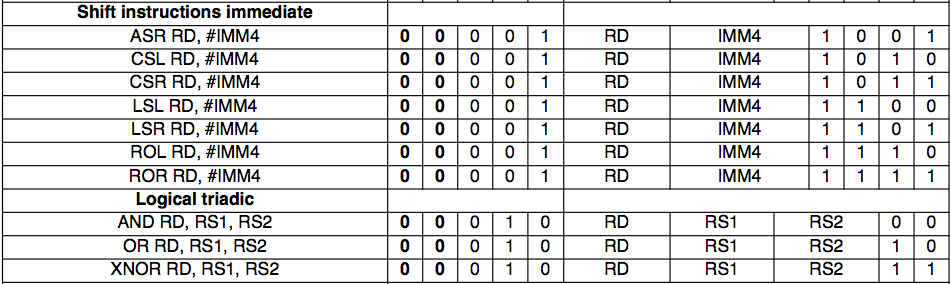
\includegraphics[width=0.95 \linewidth]{../common/images/shiftAndTriadicInstFormat.png}
    \caption{Codage binaire des instructions de décalage (shift) et les instruction triadiques (3 registres) sur la XGate. \emph{Source Freescale}}
    \label{fig:shiftAndTriadicInstFormat}
  \end{center}
\end{figure}

On peut directement remarquer sur cet exemple que le bit 12 sert à différencier les 2 types d'instructions. D'une manière plus générale sur tout le jeu d'instruction, les 5 bits de poids forts permettent d'identifier les familles d'instructions (\emph{opcode}):
\begin{lstlisting}
format inst
  select slice {15..11}
    case \b00001 is shiftInstructionImm
    case \b00010 is logicalTriadic
  end select
end format
\end{lstlisting}
Pour les instruction de déplacement avec une valeur immédiate, on définit alors le sous format \texttt{shiftInstructionImm}:
\begin{lstlisting}[firstnumber=7]
format shiftInstructionImm #IMM
  rdIndex := slice{10..8}
  imm4 := slice{7..4}
  select slice {3..0}
    case \b1001 is #ASR
    case \b1010 is #CSL
    case \b1011 is #CSR
    case \b1100 is #LSL
    case \b1101 is #LSR
    case \b1110 is #ROL
    case \b1111 is #ROR
  end select
end format
\end{lstlisting}
La signature des instructions devient alors \texttt{\#IMM \#ASR} pour l'instruction \texttt{ASR}, \texttt{\#IMM \#CSL} pour \texttt{CSL}, \ldots
Au niveau des instructions triadic, la description devient:
\begin{lstlisting}[firstnumber=20]
format logicalTriadic #Triadic
  rdIndex := slice{10..8}
  rs1Index := slice{7..5}
  rs2Index := slice{4..2}
  select slice {1..0}
    case \b00 is #AND
    case \b10 is #OR
    case \b11 is #XNOR
  end select
end format
\end{lstlisting}
Ainsi, nous avons ici décrit le format binaire de ces 10 instructions en 29 lignes.

\subsection{Génération du décodeur}
Il est possible de générer un décodeur directement, alors que les autres vues (syntaxe et behavior) ne sont pas encore décrites. Dans ce cas, il faut appeler le compilateur en précisant les options suivantes:
\begin{verbatim}
$ gadl --no-behavior --no-deasm test.hadl
\end{verbatim}
Ceci permet dans un premier temps de vérifier les erreurs syntaxiques et sémantiques de la description binaire. Il y a notamment une vérification de l'orthogonalité du jeu d'instruction, c'est-à-dire qu'un codage binaire ne peut correspondre qu'à une seule instruction. Cette vérification peut être longues (quelques secondes pour 1500 instructions) et il est possible de la désactiver une fois que la description binaire est terminée. On utilise alors l'option \texttt{--no-check}.

\subsection{Exploitation des fichiers de sortie}
En plus du décodeur (qui se trouve dans les fichiers \texttt{instDecoder.h} et \texttt{instDecoder.cpp}), un certain nombre de fichiers sont générer pour faciliter la mise au point. Tout d'abord, les fichiers \texttt{format\_all.dot} et \texttt{format\_ref.dot} permettent d'afficher l'arbre de description du format des instruction. Ces 2 fichiers sont au format GraphViz. Le premier affiche l'arbre complet (en indiquant les \emph{format} ainsi que les instruction de type \emph{select}), voir figure \ref{fig:formatAllTest}.

\begin{figure}[h]		%% format All
  \begin{center}
    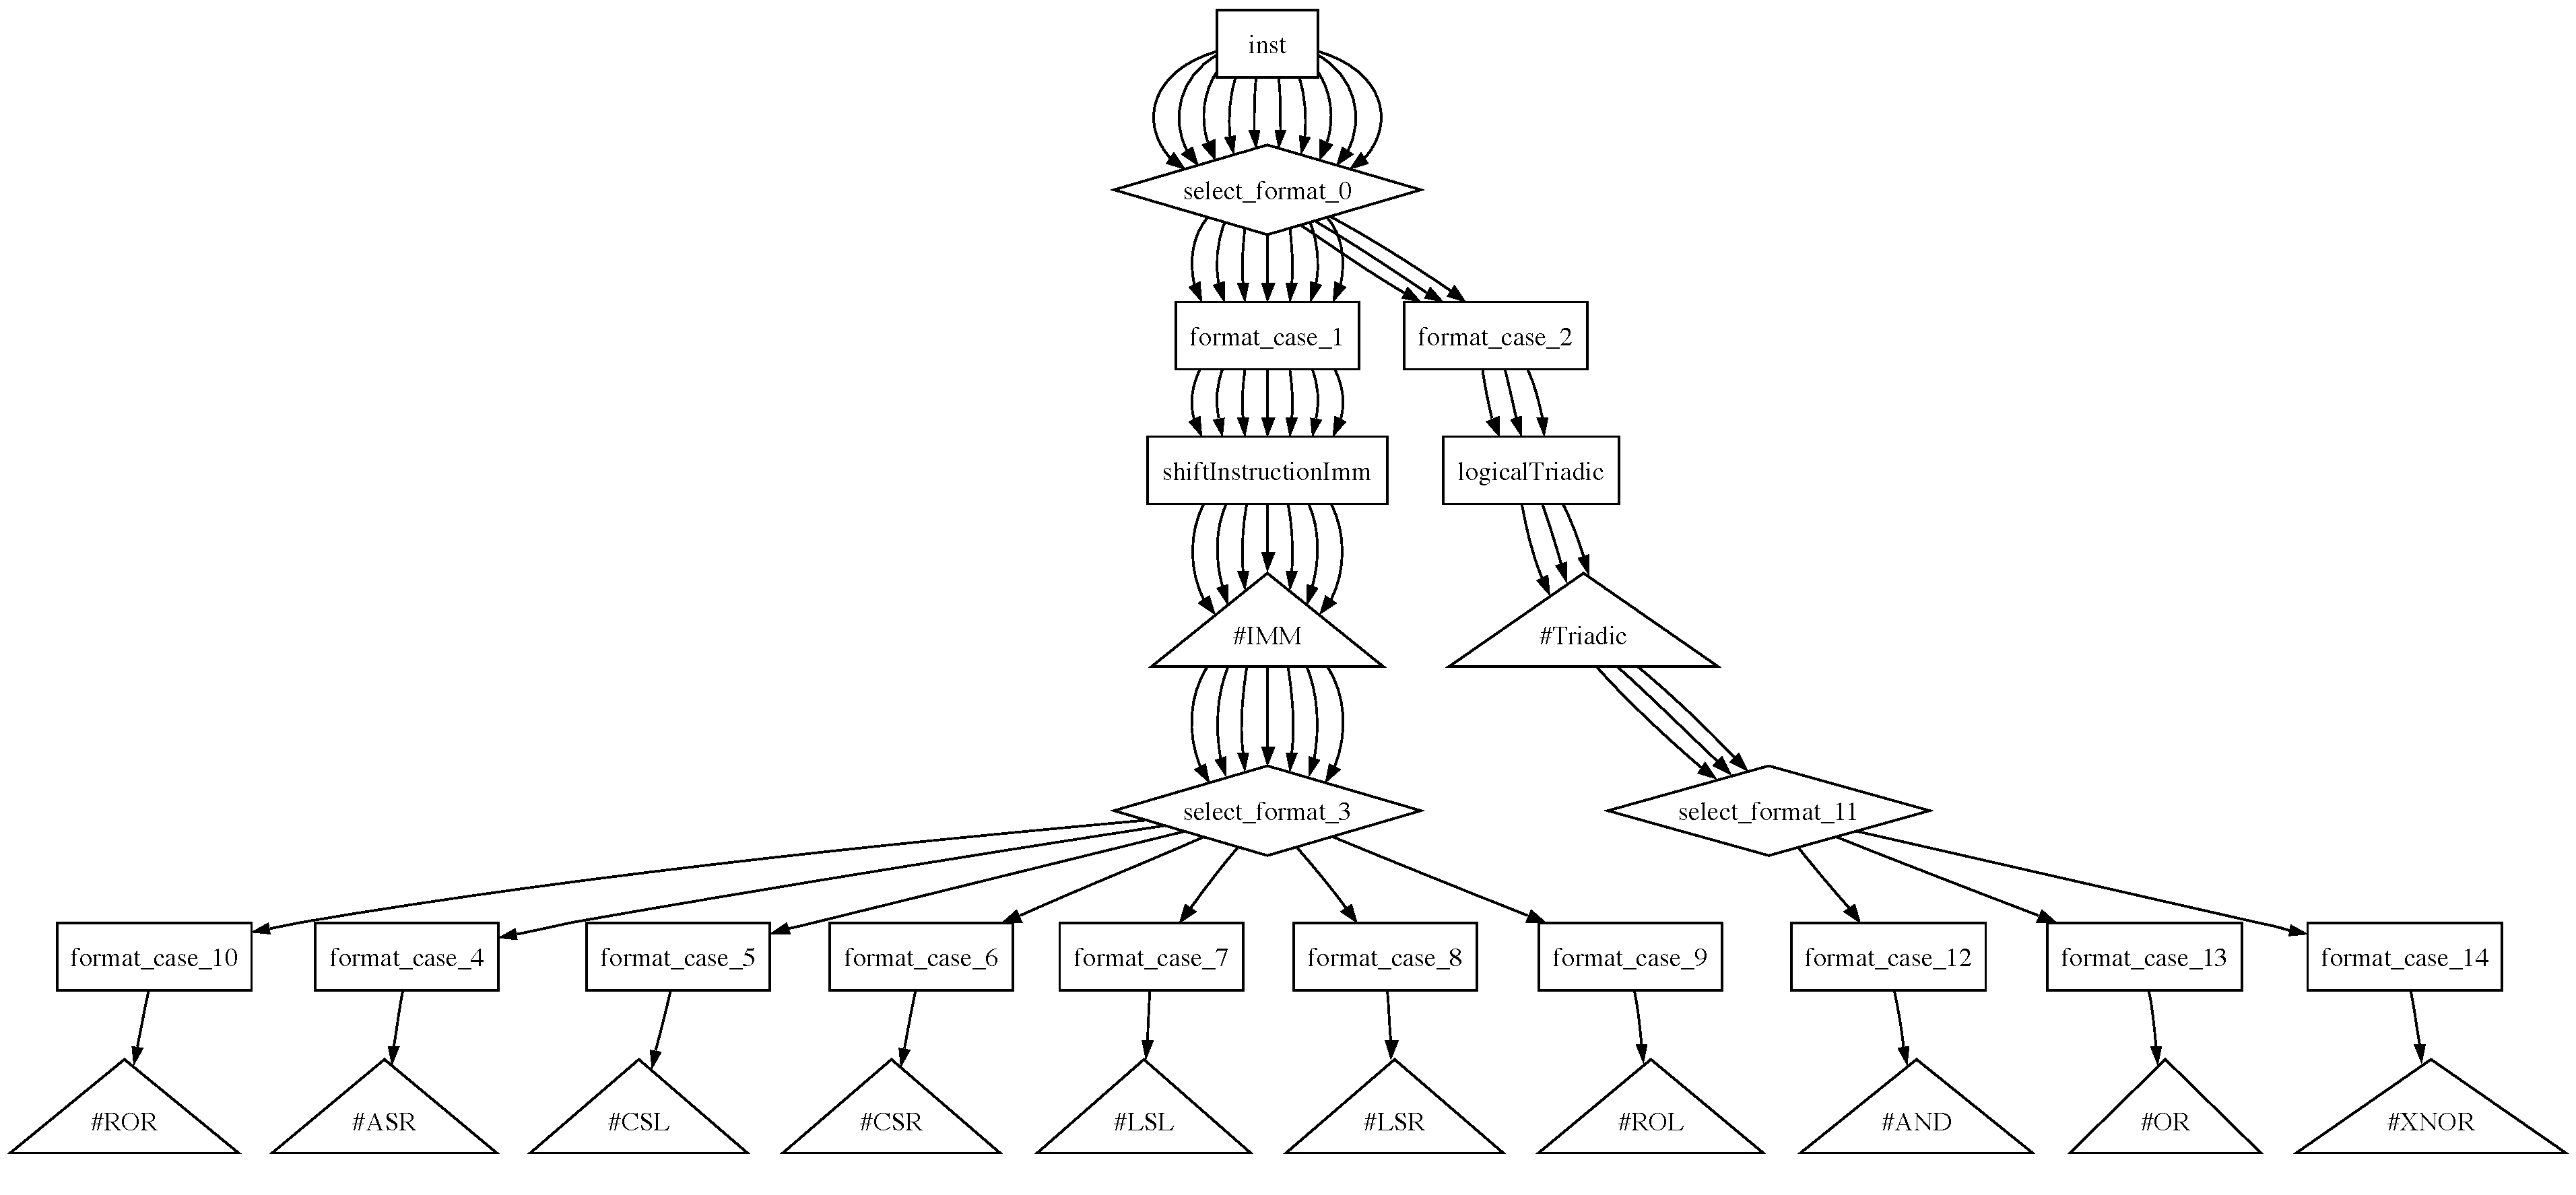
\includegraphics[width=\linewidth]{../common/images/format_all_test.pdf}
    \caption{Arbre généré à partir de la description du code binaire des instructions de décalage (shift) et les instruction triadiques (3 registres) sur la XGate.}
    \label{fig:formatAllTest}
  \end{center}
\end{figure}

Cet arbre devient vite difficile à visualiser, c'est la raison d'être du deuxième fichier qui permet d'afficher uniquement les étiquettes pour chaque instruction (voir figure \ref{fig:formatRefTest}). Dans cette dernière figure, il y a maintenant 2 structures arborescentes simples, car les instructions de décalage et les instruction triadic ne partagent pas de propriétés communes (donc pas d'étiquettes).

\begin{figure}[h]		%% format All
  \begin{center}
    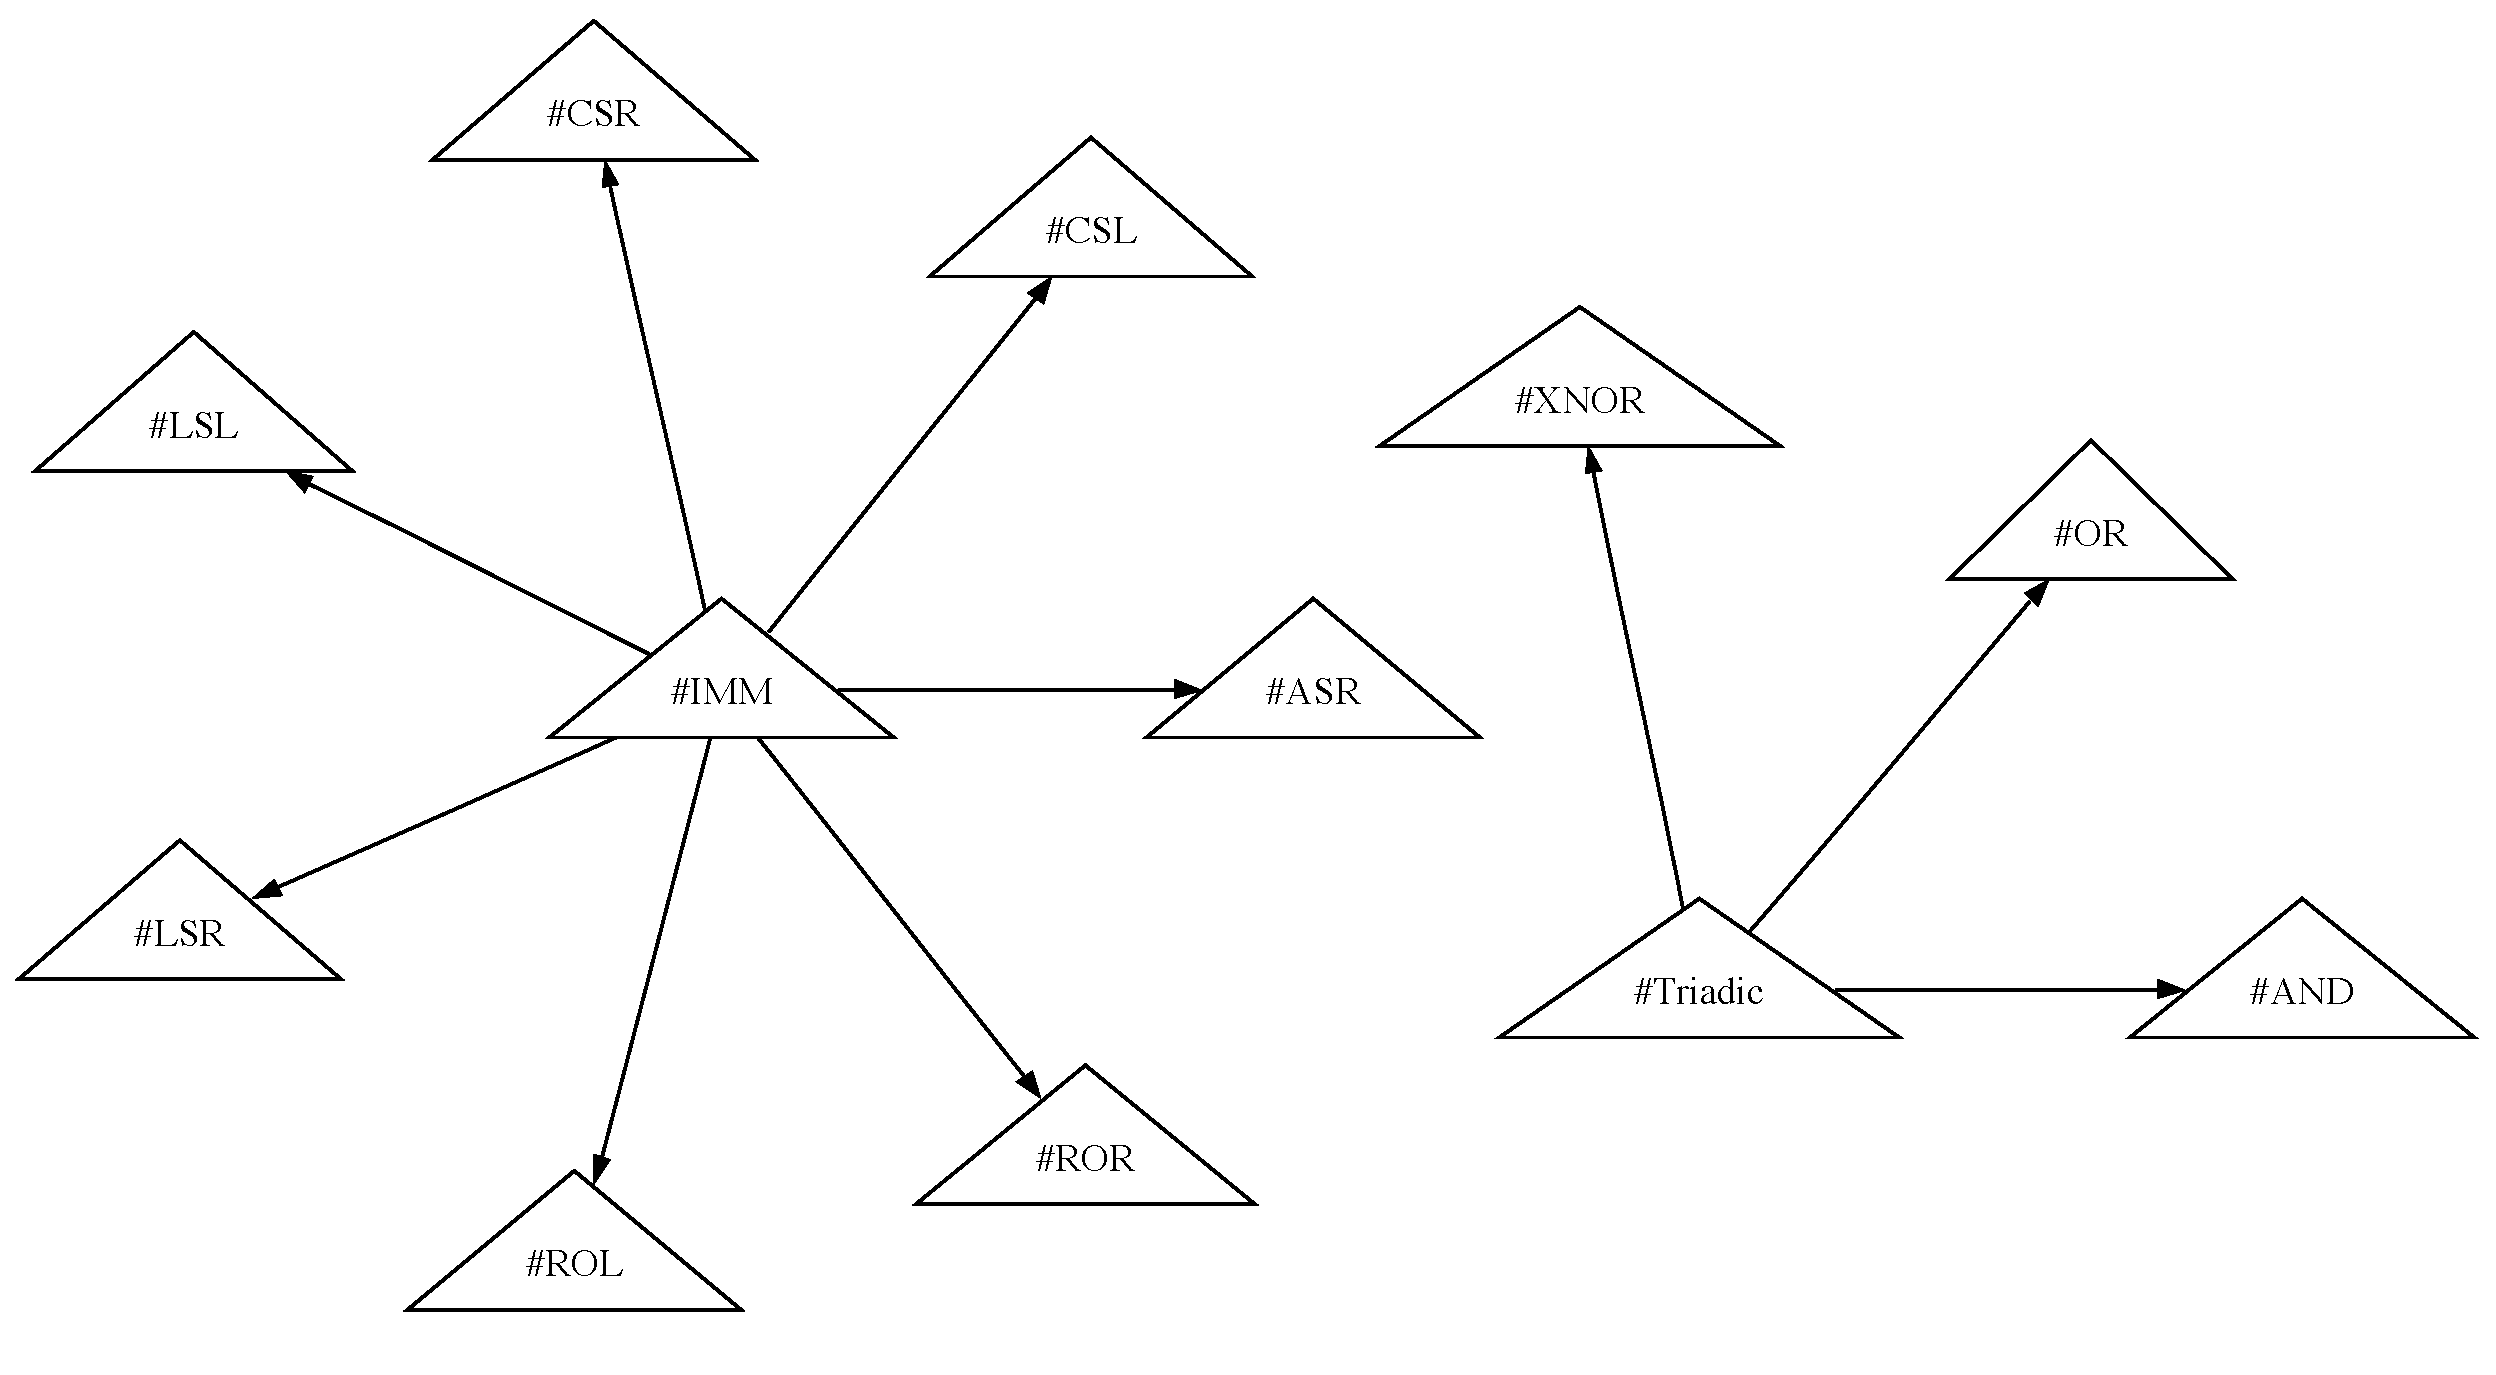
\includegraphics[width=\linewidth]{../common/images/format_ref_test.pdf}
    \caption{Arbre généré à partir de la description du code binaire des instructions de décalage (shift) et les instruction triadiques (3 registres) sur la XGate. Cet arbre est réduit aux étiquettes.}
    \label{fig:formatRefTest}
  \end{center}
\end{figure}

Enfin, en parallèle est généré un fichier qui résume les informations relatives au code binaire des instructions: \texttt{instruction.log}. On retrouve alors pour chaque instruction les informations suivantes:
\begin{itemize}
\item le parcours de l'arbre permettant de générer l'instruction;
\item la signature de l'instruction: les étiquettes sont clasées par ordre alphabétique;
\item le nom utilisé en interne par l'instruction (pour faire de la mise au point au niveau du C++ généré)
\item le codage binaire, à l'exception des champs de données
\item les noms des différents champ de données, ainsi que leur taille.
\item le code de l'instruction (en mots dont la taille est définie dans la section \emph{default});
\end{itemize}

Ainsi, on obtient par exemple pour l'instruction triadic AND les informations suivantes:
\begin{verbatim}
inst 
-> select_format_0 
-> format_case_2 
-> logicalTriadic 
-> #Triadic 
-> select_format_11 
-> format_case_12 
-> #AND
	instruction id :#AND, #Triadic
	Internal name :test_AND_Triadic
	Binary coding :00010---------00
	data field(s) :rdIndex (3 bits)
	               rs1Index (3 bits)
	               rs2Index (3 bits)
	Instruction code size :1
\end{verbatim}

%TODO: debug -> fichier de log
%intérêt de l'archi avec les codes de l'ARM.
%indiquer que les performances du décodeur ne dépendent pas de la structure de l'arbre de description.

\section{Cas des jeux d'instructions de taille variable}
\label{sec:formatTailleVariable}
Les instructions de tailles variables sont décrites en rajoutant dans les nœuds des mots, relativement aux nœuds précédents.
Soit l'exemple suivant, issu de la description du jeu d'instruction du Freescale HCS12, la taille d'un mot est de 8 bits:
\begin{lstlisting}
format Instruction 
  select slice {7..0}
    case \x18 is inst_18 
    ....
  end select
end format

format inst_18 
  select slice +{7..0}
    case \m00010111 is #CBA       -- 17h
    ...
  end select
end format
\end{lstlisting}
Dans cet exemple, le premier nœud (\texttt{Instruction}) permet de définir complètement le premier mot (comme pour les jeux d'instructions de taille fixe). Le nœud \texttt{inst\_18} est appelé si le premier mot est \texttt{0x18}. Dans le format \texttt{inst\_18}, il y a un \texttt{+} dans le select, ligne 9; ceci indique qu'il est nécessaire de rajouter un mot pour décrire le format binaire de l'instruction. Ainsi, la sémantique de \texttt{+\{7..0\}} est: \emph{on ajoute 1 mot, et on fait un \texttt{select} sur les 8 bits de ce nouveau mot.}

D'une manière plus générale, un \texttt{select} de la forme: \texttt{\{a..b\}\{c..d\}+\{e..f\}\{-\}\{g..h\}} indique que l'on rajoute 3 mots pour les instructions de la branche et que l'on fait un \texttt{select} sur:
\begin{itemize}
\item le champ \texttt{a..b} du mot précédent;
\item le champ \texttt{c..d} du mot courant;
\item le champ \texttt{e..f} du premier nouveau mot rajouté;
\item le deuxième nouveau mot n'est pas utilisé dans le \texttt{select};
\item le champ \texttt{g..h} du troisième nouveau mot rajouté;
\end{itemize}
S'il n'y a pas eu auparavant de rajout de mot (et qu'il n'y a que le mot courant), une erreur est générée car il est impossible d'accéder au mot précédent.

Si un nouveau format est appelé dans, ou après le \texttt{select}, le dernier mot rajouté devient le mot courant.

Cette approche par accès relatif (on rajoute un mot au mot précédent) permet de résoudre aisément les instructions dont le moe d'adressage n'est pas toujours sur le même mot, comme dans l'exemple de la figure \ref{fig:formatLongueurVariable}.
\begin{figure}		%% Small Example
  \begin{center}
    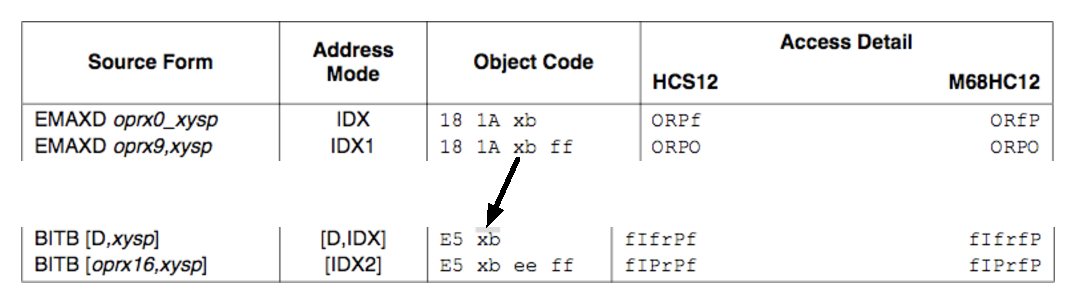
\includegraphics[width=0.8 \linewidth]{../common/images/formatLongueurVariable.pdf}
    \caption{Exemple de formats de données de longueur variable, issue de la documentation du HCS12. Le mode d'adressage \texttt{xb} peut-être à différentes places. (source Freescale).}
    \label{fig:formatLongueurVariable}
  \end{center}
\end{figure}

%TODO: rajouter le fetch explicite!!!